\chapter{Pendahuluan}
\label{chap:pendahuluan}

\section{Latar Belakang}
\label{sec:latar_belakang}

KIRI (\url{http://kiri.travel}) adalah sebuah situs yang dikelola oleh PT. Kirana Sistem Transportasi, yang menyediakan layanan navigasi dari satu titik ke titik lain memanfaatkan transportasi publik. Layanan ini diberikan secara gratis kepada pengunjung situs / pengguna aplikasi bergerak mereka. Untuk mendukung layanan tersebut, tim KIRI melakukan kurasi rute angkot secara mandiri di Bandung dengan mencatat perjalanan setiap trayek menggunakan peralatan GPS (\textit{Global Positioning System}). Pada perkembangannya, KIRI melakukan ekspansi ke beberapa kota lainnya termasuk Jakarta. Hanya saja, karena keterbatasan sumberdaya data di Jakarta dimasukkan berbekal data yang tersedia di internet, tanpa validasi di lapangan. Di sisi lain, ada beberapa pihak yang tertarik akan layanan KIRI di Bandung dan berniat untuk mendapatkan layanan serupa di kota mereka. Tampilan situs web KIRI dapat dilihat pada gambar \ref{fig:1_kiri}.

\begin{figure}
	\centering
	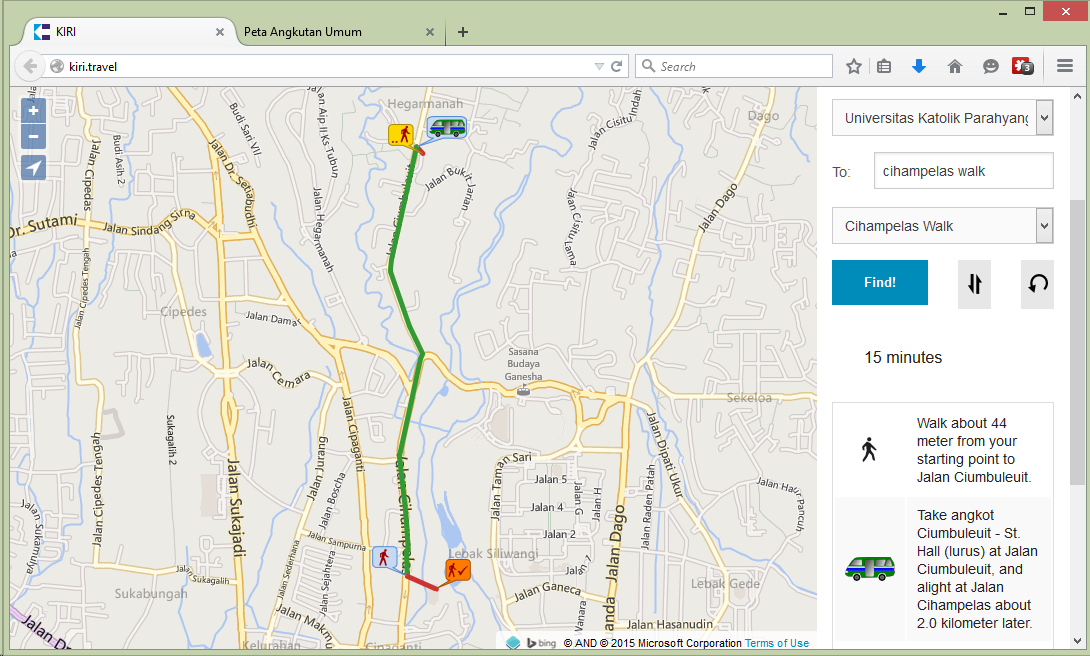
\includegraphics[scale=0.5]{Gambar/1_kiri}
	\caption{Situs Web KIRI} 
	\label{fig:1_kiri}
\end{figure}

Situs \url{https://angkot.web.id} (selanjutnya disebut angkot.web.id saja) merupakan sebuah situs yang dikembangkan oleh Fajran Iman Rusadi yang berbasis di Belanda. Situs ini memungkinkan pengguna publik untuk melihat, memasukkan, atau memperbaiki data rute angkot di Indonesia (dengan kata lain, \textit{crowdsourcing}). Layanan ini juga diberikan secara gratis. Tampilan situs web angkot.web.id dapat dilihat pada gambar \ref{fig:1_angkotwebid}

\begin{figure}
	\centering
	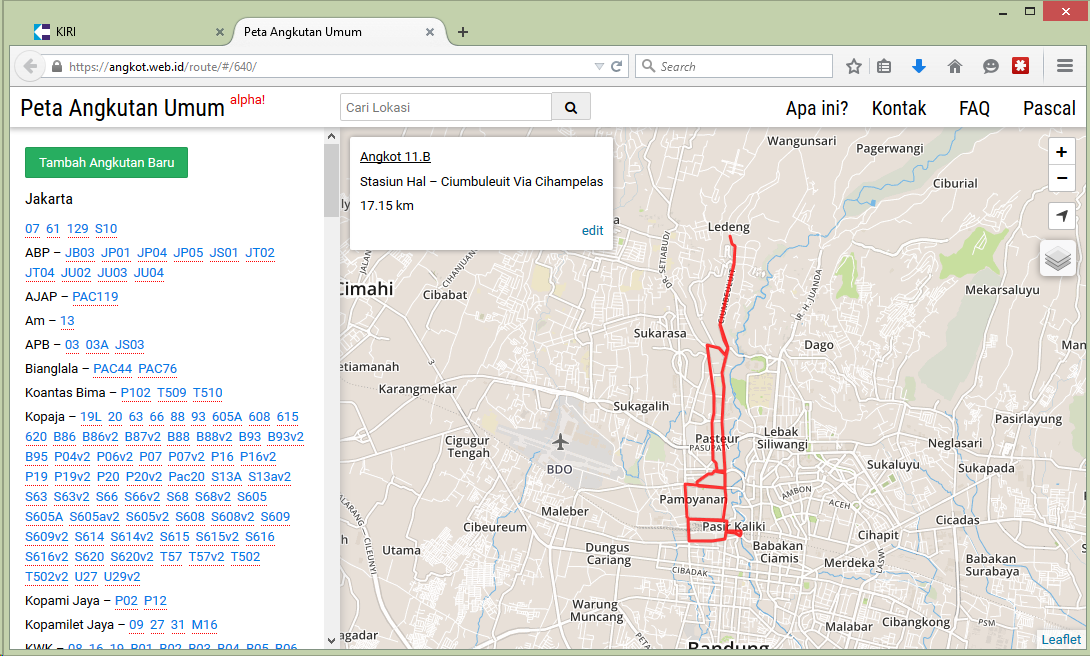
\includegraphics[scale=0.5]{Gambar/1_angkotwebid}
	\caption{Situs angkot.web.id}
	\label{fig:1_angkotwebid}
\end{figure}

Sampai saat ini, KIRI serta angkot.web.id merupakan dua buah situs yang terpisah dan bekerja secara independen.

\section{Rumusan Masalah}
\label{sec:rumusan_masalah}
Dari latar belakang yang sudah dijelaskan, peneliti bermaksud untuk mengintegrasikan data yang dimiliki kedua situs web tersebut. Integrasi tersebut dirumuskan ke dalam masalah-masalah berikut:
\begin{enumerate}
	\item Bagaimana mekanisme penarikan data oleh KIRI terhadap angkot.web.id secara otomatis?
	\item Bagaimana memisahkan data yang dimiliki oleh KIRI sendiri dengan data yang ditarik dari angkot.web.id?
	\item Bagaimana mengoptimasi protokol yang digunakan, sehingga kebutuhan \textit{bandwidth} dapat dihemat?
	\item Bagaimana respon pengguna KIRI terhadap fitur yang diimplementasikan?
\end{enumerate}

\section{Tujuan}
\label{sec:tujuan}
Berdasarkan rumusan masalah yang sudah dijabarkan, maka didefinisikan tujuan-tujuan berikut:
\begin{enumerate}
	\item Mengimplementasikan mekanisme penarikan data otomatis oleh KIRI terhadap angkot.web.id.
	\item Mengimplementasikan pemisahan data antara rute milik KIRI dengan data yang ditarik dari angkot.web.id.
	\item Mengoptimasi protokol yang digunakan, sehingga kebutuhan \textit{bandwidth} dapat dihemat.
	\item Mempelajari respon pengguna KIRI terhadap fitur yang diimplementasikan.
\end{enumerate}

\section{Batasan Masalah}
\label{sec:batasan_masalah}
Penelitian ini memiliki batasan-batasan seperti berikut:
\begin{enumerate}
	\item Penelitian dilakukan untuk rute angkot kota Bandung saja.
	\item Dengan alasan kerahasiaan, penelitian ini tidak membahas keseluruhan bagian dari KIRI dan angkot.web.id, melainkan hanya bagian yang penting saja.
\end{enumerate}

\section{Metode Penelitian}
\label{sec:metode_penelitian}
Dalam penelitian ini, akan dilakukan langkah-langkah berikut:
\begin{enumerate}
	\item Melakukan studi terhadap mesin navigasi KIRI, protokol angkot.web.id, serta teori-teori lain yang mendukung kedua hal tersebut.
	\item Melakukan analisis untuk menemukan hal yang dapat dilakukan untuk mengintegrasikan data kedua situs tersebut.
	\item Melakukan perancangan untuk implementasi integrasi kedua sistem tersebut.
	\item Melakukan implementasi dari rancangan yang sudah dilakukan.
	\item Melakukan publikasi terhadap pengguna KIRI sehingga mereka dapat menguji hasil implementasi tersebut.
	\item Menganalisa dan menarik kesimpulan atas hasil penelitian yang telah dilaksanakan.
\end{enumerate}

\section{Sistematika Penulisan}
\label{sec:sistematika_penulisan}
Berikut adalah sistematika penulisan dari dokumen ini:
\begin{itemize}
	\item Bab 1 membahas latar belakang, rumusan masalah, tujuan penulisan, batasan-batasan, serta metode yang digunakan pada penelitian ini.
	\item Bab 2 membahas teori-teori yang digunakan dalam penelitian ini.
	\item Bab 3 membahas analisis yang dilakukan terhadap teori yang telah dijabarkan pada bab 2.
	\item Bab 4 membahas perancangan yang dilakukan sebelum mengimplementasikan integrasi yang dimaksud.
	\item Bab 5 membahas implementasi serta pengujian dari integrasi yang telah dilakukan.
	\item Bab 6 membahas kesimpulan dari keseluruhan penelitian ini, serta saran-saran yang dapat diberikan untuk penelitian berikutnya.
\end{itemize}